\chapter[Plot Outputs]{PLOT OUTPUTS}
\label{plot}

{\sl FEAPpv} provides for the construction of plots to represent features of
the problem and its solution.
This section contains specific instructions for constructing graphical
views for a solution.

\section{Screen Plots}
\label{screen}

{\sl FEAPpv} presents graphics to the screen when starting the program.
Options include an X-window mode and a PC-window mode.
Plots are constructed using commands,
similar to those described above for problem solution, and
may be performed in a batch mode as
\begin{verbatim}
       Macro> PLOT,command,options
\end{verbatim}
or in an interactive mode by first issuing the command
\begin{verbatim}
       Macro> PLOT
\end{verbatim}
followed by the sequence of plot commands to be executed
(for clarity, a prompt indicating the solution mode is shown before each
command; however, only the command is entered by the user).  When in the
interactive mode the {\tt PLOT} is not issued as part of the command.
Thus, the command
\begin{verbatim}
       Plot> MESH
\end{verbatim}
will display the mesh. The interior of each element may be filled in a color
by giving the command
\begin{verbatim}
       Plot> FILL
\end{verbatim}
The color for different materials will be selected based on its material number.
Additional options may exist for these and subsequent commands as described in
Appendix C; however, below some of the options to construct basic plots are
described.

To place the nodes on the screen while in interactive mode only the command
\begin{verbatim}
       Plot> NODE
\end{verbatim}
is given.  To place the number for node 5 only, the command
\begin{verbatim}
       Plot> NODE,5
\end{verbatim}
is used.  Similarly, all element numbers are placed on the mesh using the
commands {\tt ELEMent} or {\tt ELEMent,4}
to get all elements or only element 4, respectively.

A perspective view of any mesh may be constructed using the command
{\tt PERSpective}.  For three dimensional problems, the command {\tt HIDE}
should be used to develop all plots on the visible surfaces.  To return to
the original Cartesian form of plots the command {\tt CARTesian} is used.

Features may be added to mesh plots by using other commands.
An outline of a mesh may be displayed using the command {\tt OUTLine}.
To display the
boundary conditions for degree-of-freedoms 1 to 3 the command {\tt BOUN}
may be used.  Alternatively, any individual directions restraints may be
shown using {\tt BOUN,dir}, where {\tt dir} ranges from 1 to 3.  At present,
boundary conditions for degree-of-freedoms greater than 3 may only be displayed
using the \texttt{BOUN,dir} form.

Once a solution is performed using the command language features described
in Chapter \ref{command} it is possible to display several features of
the solution.  Vectors of the nodal generalized displacements may be shown
using the command {\tt DISP}lacement.  Contours of the displacements are
constructed using {\tt CONTour,dof} where {\tt dof} is the number of the
displacement to contour.  A range of values will be selected and if a
default mode is in effect the contours will be placed on the screen.  If
the default mode is inactive it is necessary to select the plot ranges (default
values are suggested and may be accepted by using the enter key).  The
default mode may be turned on and off in interactive mode using the
commands {\tt DEFAult,ON} and {\tt DEFAult,OFF}, respectively.

Contours of element variables, such as stresses, may be constructed using
the command {\tt STREss,comp} where {\tt comp} is the component to be plotted.
For {\sl FEAPpv} solid elements the stress components are ordered as shown in
Table \ref{tab18a}.

\begin{table}
\begin{center}
\begin{tabular}{| c | l |} \hline
COMP & Description \\ \hline
1 & 11-Stress \\
2 & 22-Stress \\
3 & 33-Stress \\
4 & 12-Stress \\
5 & 23-Stress \\
6 & 31-Stress \\ \hline
\end{tabular}
\caption{Component number for solid element stress value}
\label{tab18a}
\end{center}
\end{table}
To construct contours the stress values are first projected to the nodes.
For two-di\-men\-sion\-al meshes it is also possible to show the unprojected
stress contours using the {\tt ESTRess,comp} command.
Projected principal values of stresses
may also be displayed using the command {\tt PSTRess,comp}
where the components are ordered as shown in Table \ref{tab18b}

\begin{table}
\begin{center}
\begin{tabular}{| c | l |} \hline
COMP & Description \\ \hline
1 & 1-Principal Stress \\
2 & 2-Principal Stress \\
3 & 3-Principal Stress \\
4 & Maximum Shear (2-D) \\
5 & $I_1$-Stress Invariant\\
6 & $J_2$-Stress Invariant\\
7 & $J_3$-Stress Invariant\\ \hline
\end{tabular}
\caption{Component number for solid element principal stress value}
\label{tab18b}
\end{center}
\end{table}
The directions of the principal axes at nodes may be shown using the
command {\tt PRAXis}.

It is also possible to show all of the above
plots on a deformed position of the mesh by using the command
\begin{verbatim}
       DEFOrm,factd,freeze,facte
\end{verbatim}
before giving any of the above commands.  The parameters {\tt factd} and
{\tt facte} are scale factors for displacements and eigen-vectors, respectively.
A non-zero value for the parameter {\tt freeze} will keep the values of
original scaling distances and, thus, permits a deformed mesh over an undeformed
mesh with the same scaling.  Similarly, the command {\tt UNDE,,freeze} returns
plots to an undeformed configuration without rescaling the plot.

To plot an eigen-vector it is necessary to provide the {\tt facte} scaling using
the {\tt DEFOrm} command before issuing the eigen-vector plot command
{\tt EIGVector,num} where {\tt num} is the number of the vector to plot.
The ordering for {\tt num} is the same as that for the eigen-values computed
by the {\tt SUBS}pace solution command.

In interactive mode it is possible to select a part of the mesh region for
displaying plotted quantities.  This is performed using the command {\tt PICK}
and then the mouse to select two points bounding the region to be plotted.  
The points selected will be used to construct a square region and, thus,
may be slightly different than selected.  To return to a full mesh plot
use the command {\tt ZOOM}.

\section{PostScript Plots}
\label{postscript}

{\sl FEAPpv} provides for construction of files in the encapsulated 
PostScript format.  To
construct a PostScript file for graphics output the command {\tt POST}
is given.  The first time the command is used a file is opened and
named.  The name of the file is {\tt feapx.eps},
where {\tt x} is a letter between
the lower case {\tt a} and the upper case {\tt Z} (52 files may be made -
only
26 in PC mode since the difference in upper and lower cases is ignored).
Information for all commands issued after the {\tt POST} command will appear
both on the screen device and in the file.  The second time the command is
given the PostScript file is closed.  If another pair of {\tt POST} commands
are issued a new file will be created and closed.  The files may be converted
to hard copy in a UNIX environment using the {\tt lpr} command.

PostScript files may be created in either a portrait or landscape mode.
In addition, the {\sl FEAPpv} logo is normally not placed in the file.

One example of using the PostScript options is a mesh plot and load
for a given problem.  For two-dimensional applications the 
set of commands:
\begin{verbatim}
       PLOT,POSTscript    !open a file to accept plot data
       PLOT,MESH          !plot mesh
       PLOT,LOAD,,-1      !plot load with tip on nodes
       PLOT,POSTscript    !close file
\end{verbatim}
produces a file containing the mesh and load.
This is the set of commands which produced Figure \ref{fig71}.
If desired the location of the origin of the coordinate axes may be
displayed using the command {\tt AXIS}.  If the origin is outside the
plot window the axes will not appear.  It is possible to relocate the
axes by giving the command
{\tt AXIS,x,y,z} where the x,y,z are dimensions in terms of
the mesh coordinates.

In three dimensions it is
usually preferable to select a perspective type plot and view options
and then produce
surface plots which {\it hide} parts of the mesh not visible.  Thus, prior
to issuing the graphical output
commands one should issue the plot command sequence:
\begin{verbatim}
       PLOT,PERSpective   ! requires view information
       PLOT,HIDE          ! hides interior surfaces.
\end{verbatim}
See the plot manual in Appendix C
for more information on specifying the perspective view data.

\begin{figure}[ht!]
\centerline {\hfil 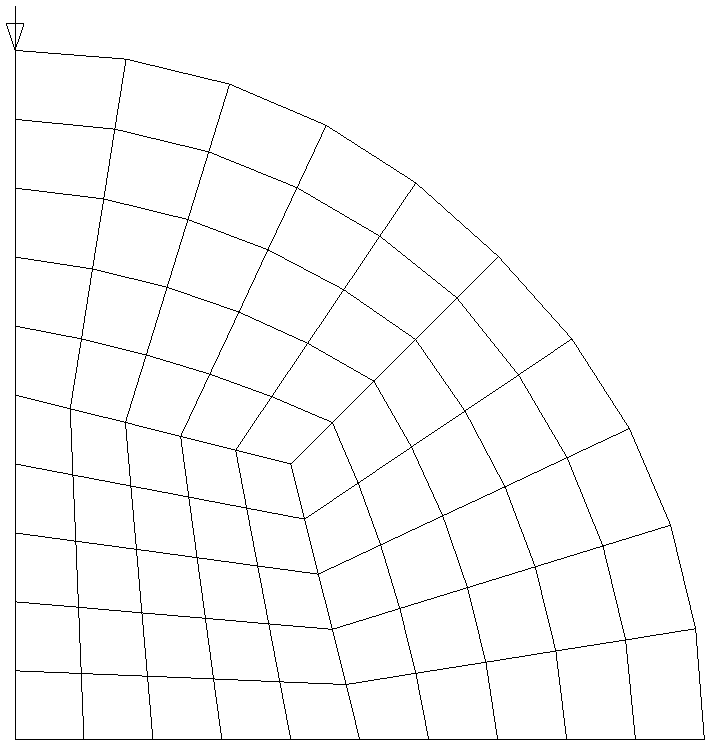
\includegraphics[width=2.8in]{figs/fig4} \hfil}
\caption{Mesh for Circular Disk. 75 Elements}
\label{fig7}
\end{figure}

After a solution has been computed, a PostScript file for
contour plots may also be obtained.
The contours of the vertical displacement for the example problem with the
mesh shown in Figure \ref{fig7} may be constructed by issuing the commands:
\begin{verbatim}
       PLOT,POSTscript    !open a file to accept plot data
       PLOT,CONT,2        !plot contours for dof 2
       PLOT,LOAD,,1       !plot load with tip on nodes
       PLOT,POSTscript    !close file
\end{verbatim}
The {\tt CONT}our command places the contours for degree-of-freedom 2, while
the {\tt LOAD} places the non-zero loads on the nodes.
The results from this sequence are shown in Figure \ref{fig8}.
To get contours for the velocity or acceleration the {\tt CONT}our command
is replaced by {\tt VELO}city or {\tt ACCE}leration, respectively.

\begin{figure}
\centerline {\hfil 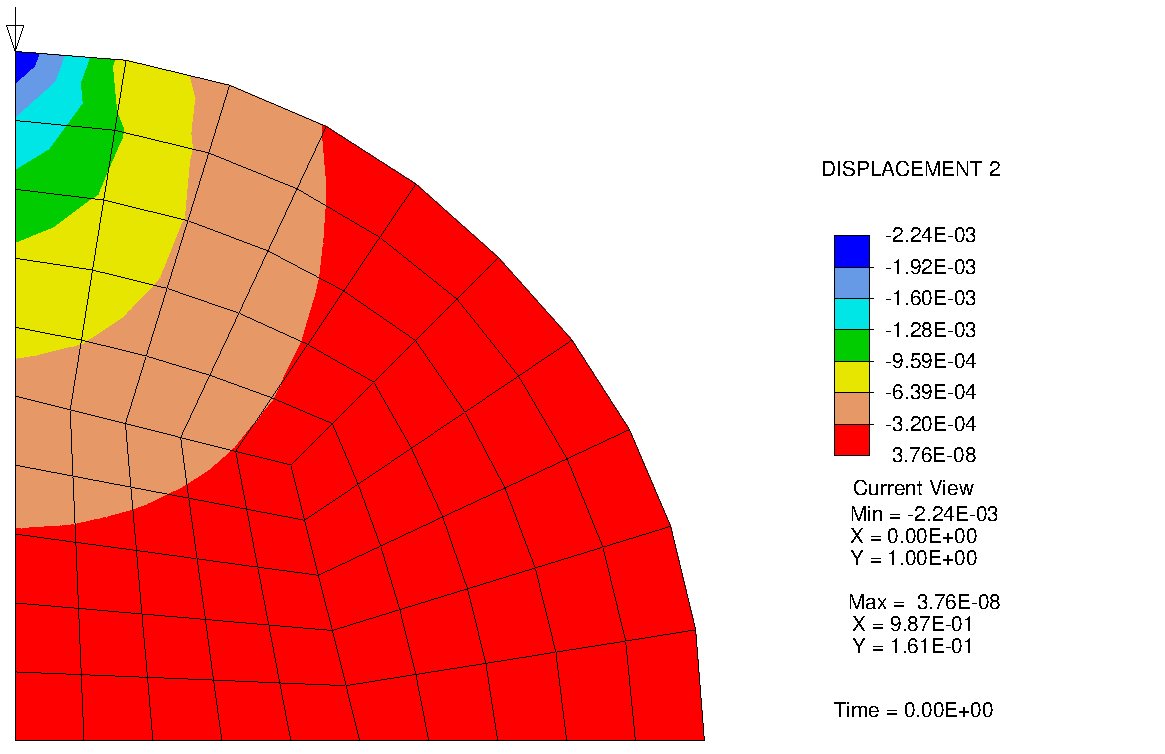
\includegraphics[width=4.8in]{figs/fig5} \hfil}
\caption{Contours of Vertical Displacement for Circular Disk}
\label{fig8}
\end{figure}

While the above examples are shown for a {\tt BATCh} execution, the same
sequence may be given from an {\tt INTEractive} execution.  That is,
while in an interactive mode issue the command {\tt PLOT} and the prompt
\begin{verbatim}
       Plot>
\end{verbatim}
will appear in the command window.
The plot sequence can then be issued one at a time.  If any
data is required, prompts may be given for the required input
Usually, defaults are suggested and may be accepted by pressing the enter key.
The need to specify parameters depends on
settings of parameters at installation time.
It may be necessary to disable or enable use of defaults using the command
\begin{verbatim}
       DEFAult,<ON,OFF>
\end{verbatim}
where either {\tt ON} or {\tt OFF} is selected to enable or disable prompts,
respectively
{\footnote{Note: The {\tt DEFA}ult command is at the intermediate level
and will not appear if the {\tt HELP} command is given at the basic level
(i.e., {\tt MANU}al= 0).}}.
At installation time it is possible to have the parameter defaults either
enabled or disabled.
The need to specify parameters depends on
settings of these parameters at installation time.
